The system has shown remarkable progress since its first creation. 
The Blender Python environment has demonstrated its ability to act as an effective programming tool for creating and running 3D simulations in a quick and accurate manner. 
Our small library of functions and predications has given us a grounding from which a more extensible and complex system can be built. 

Our project has demonstrated the ability to accurately place objects and query scenes based on given predications.
Experiments in the past have demonstrated that the \TDS can, given input objects and relations, generate appropriate scenes. The following three objects were used for the majority of the tests and examples for this project:
\begin{center}
	\begin{itemize}
		\item ball ``A''
		\item snowman ``B''
		\item person ``C''
	\end{itemize}
\end{center}
these three objects were chosen because of their increasing number of mesh objects. The ball only has one mesh. 
The snowman has three meshes (the top, bottom, and middle spheres). The person, however, has fifteen meshes. 
This spectrum allows for a broad analysis of the different sized objects, which is important as certain methods' run-time is dependent on the number of mesh objects in the specified entity.
\begin{figure}[h]
	\centering
		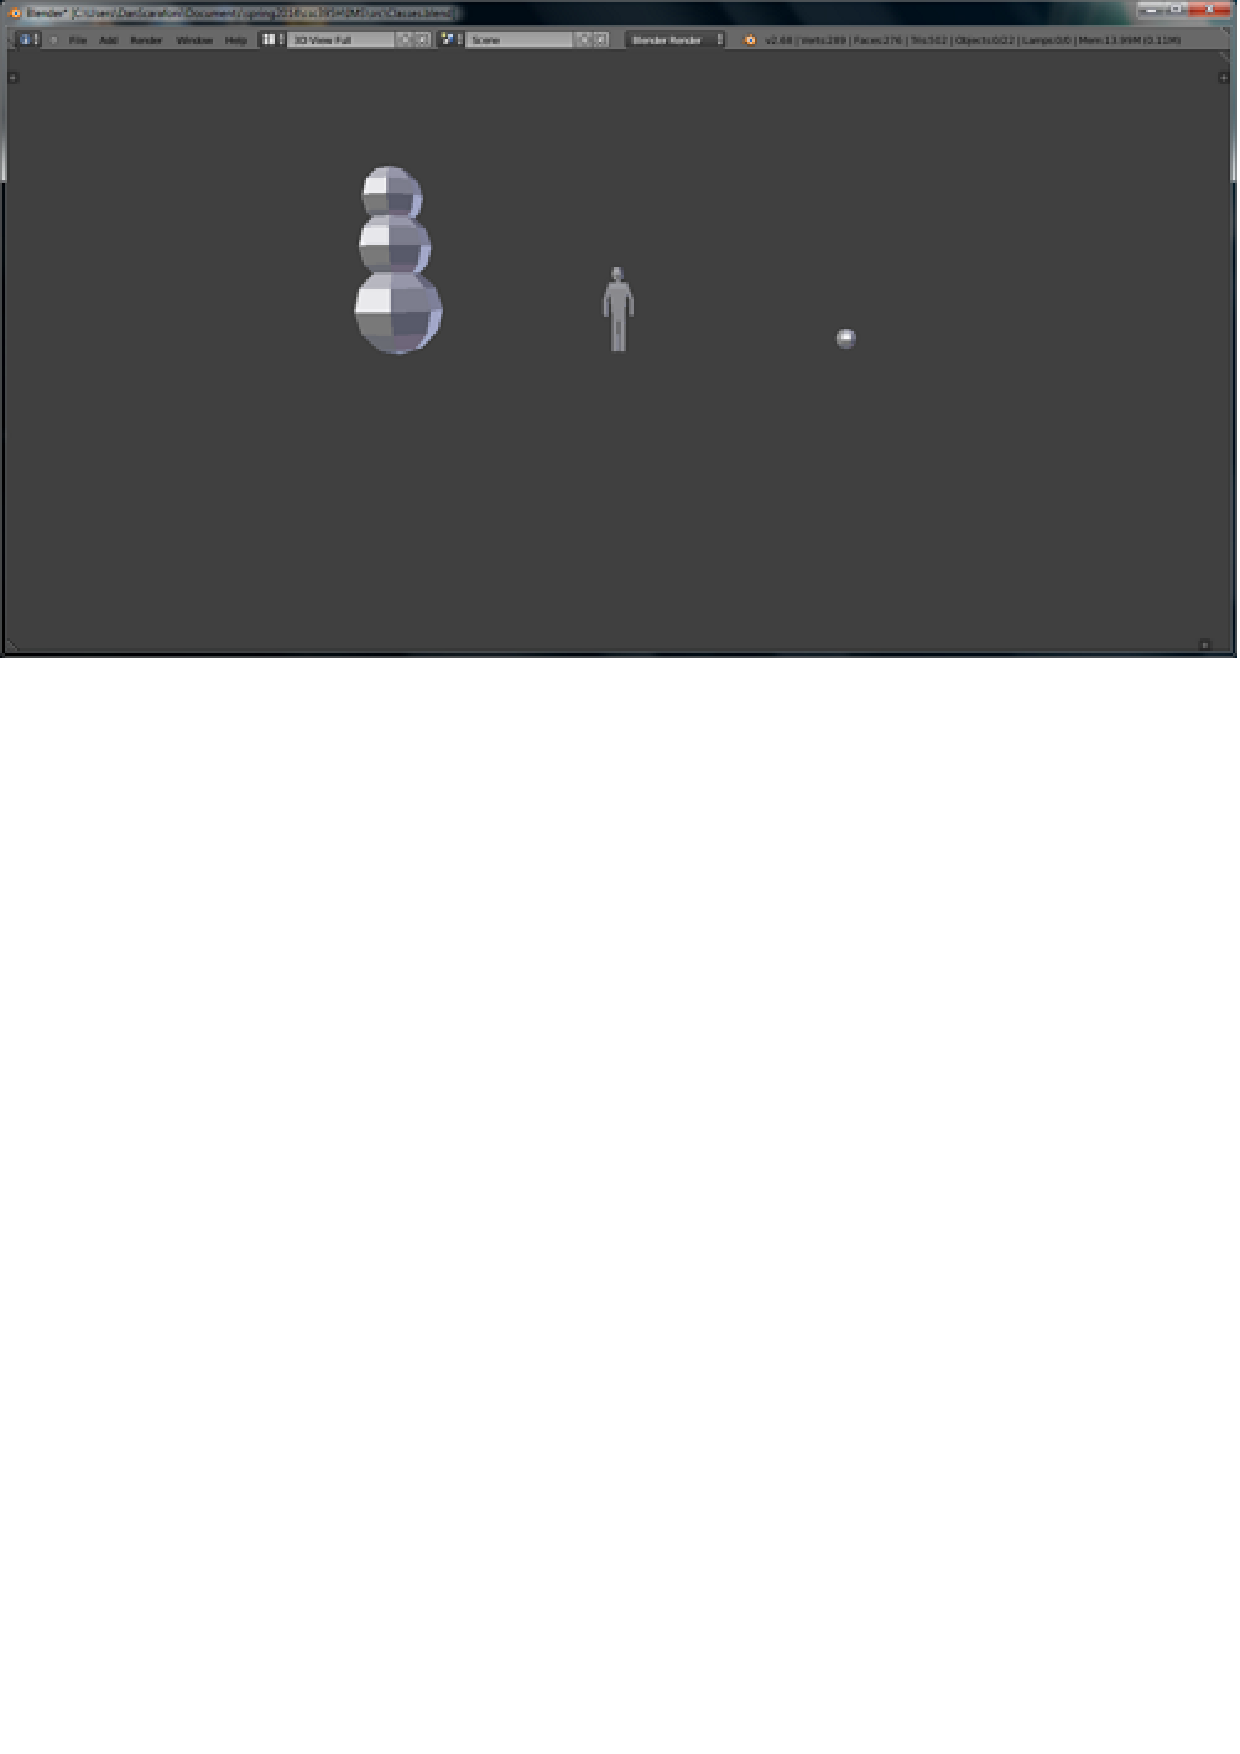
\includegraphics[width=0.48\textwidth]{figures/models_used.pdf}
	\vspace{-6cm}
	\caption[width=0.5\textwidth]{a visualization of the three objects used for basic testing. From left to right: the snowman, the person, and the ball. Entities are shown to scale.}
	\label{fig:models_used}
\end{figure}

Figure \ref{fig:models_used} provides a visualization of the three objects used. Note, however, that in the majority of testing situations, only person and ball were used.
With these objects, the program will correctly an appropriate scene which is consistent with the constraints. 
The scene for this example is seen below in figure \ref{fig:scene_demo}.
\begin{figure}[h]
	\centering
		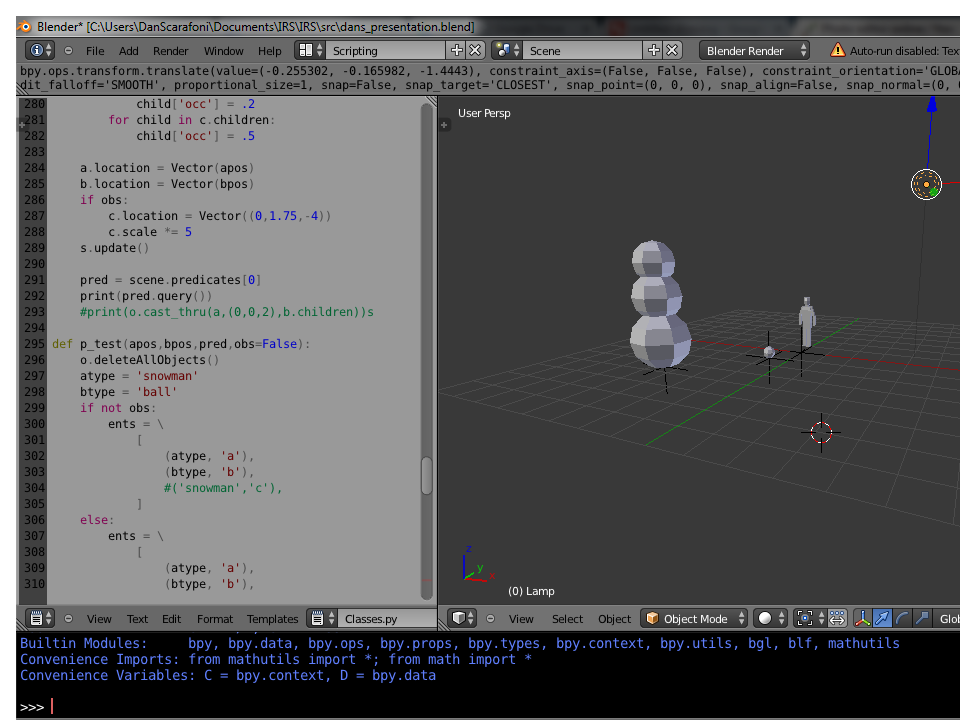
\includegraphics[width=1\textwidth]{figures/scene_demo.png}
	\caption{Given the above predicates, the \TDS
	 is able to generate an appropriate scene.}
	\label{fig:scene_demo}
\end{figure}

\section{Binary Query Tests}
The first set of tests examined the \TDS's ability to place and query based on the simple binary predicate relations. 
For these tests, only two objects were needed, and as such the person, ``B'' and ball, ``A'' were implemented (as they utilized the most and least meshes respectively).
Each predicate was tested ten times. 
In each test, the system placed the two objects were placed under the constraint \texttt{\textless predicate \textgreater (A,B)}.

An objects focality determines, in a loose sense, its importance in a scene. For the intents and purposes of this experimentation, a non-focal object is placed around a focal object. For example, for the placement of ``near(A,B)'', if object ``A'' is focal, then it is left in its original location, and object ``B'' is placed around it. The focality was varied so that testing would not improperly bias certain conditions in the placement function.

Five tests were done with the person as the \emph{focal object} (the stationary one), and five were done with the ball as the \emph{focal object}.
This gave an accurate view of the run-time of the predicates on objects of varying complexity.
These ten tests were repeated not only for every predicate, but for varying positions as well. 

The non-focal object was placed 1, 2, and 5 blender units on the x axis away from the \emph{focal object}.
The \emph{focal object} was constrained to the origin.
This was done to tests the predicates under multiple degrees of satisfiability.
For predicates such as ``above'' and ``under'' the non-focal object was also placed above and below the \emph{focal object} respectively.
If this was not done, then neither of these predicates would be satisfiable in any tests.
\begin{table}[h]
	\centering
	\begin{tabular}{|l | c | c | c | c | c |}
		\hline
		\multirow{3}{*}{predicate} & \multirow{3}{*}{distance} & \multirow{3}{*}{query} &  \multicolumn{2}{c|}{time} \\\cline{4-5}
		&  &  & average & standard deviation \\\hline
		\multirow{3}{*}{\texttt{near}} & 1 & 1 & 0.0142 & 0.005 \\\cline{2-5}
		& 2 & 1 & 0.0186 & 0.006 \\\cline{2-5}
		& 5 & 0.365 & 0.0165 & 0.006 \\\hline
		\multirow{3}{*}{\texttt{under}} & 1 & 0 & 0.0195 & 0.0 \\\cline{2-5}
		& 2 & 0 & 0.0196 & 0.004 \\\cline{2-5}
		& 5 & 0 & 0.0196 & 0.000 \\\hline
		\multirow{3}{*}{\texttt{in}} & 1 & 1 & 0.0235 & 0.005 \\\cline{2-5}
		& 2 & 0 & 0.0196 & 0.000 \\\cline{2-5}
		& 5 & 0 & 0.0227 & 0.005 \\\hline
		\multirow{3}{*}{\texttt{inside}} & 1 & 0.451 & 0.327 & 0.008 \\\cline{2-5}
		& 2 & 0 & 0.3383 & 0.016 \\\cline{2-5}
		& 5 & 0 & 0.3524 & 0.017 \\\hline 
		\multirow{3}{*}{\texttt{above}} & 1 & 0 & 0.0255 & 0.007 \\\cline{2-5}
		& 2 & 0 & 0.0264 & 0.009 \\\cline{2-5}
		& 5 & 0 & 0.0257 & 0.007 \\\hline 
		\multirow{3}{*}{\texttt{isTouching}} & 1 & 0.019 & 0.0057 & 0.004 \\\cline{2-5}
		& 2 & 0 & 0.0066 & 0.006 \\\cline{2-5} 
		& 5 & 0 & 0.0079 & 0.006 \\\hline 
		\multirow{3}{*}{\texttt{canSee}} & 1 & 1 & 0.0223 & 0.007 \\\cline{2-5}
		& 2 & 1 & 0.0182 & 0.003 \\\cline{2-5}
		& 5 & 1 & 0.0142 & 0.007 \\\hline 
	\end{tabular}
	\caption{Query Results Over Varying Predicates and Distances.}
	\label{table:query_results}
\end{table}

Because of the increased complexity of the ``canSee'' predicate, customized testing is necessary. 
To accurately gauge the efficacy of this predicate, the following scenario was used: a ball was placed in the coordinate origin. 
Around it, the person model was placed at one of eight locations: five blender units above or below on both the x and y axis.
An obscuring snowman was placed at the coordinates \texttt{(3,0,0)} so that the line of sight between the person and the ball would be obscured when the person was placed in front of the snowman.
The snowman was given an occluding factor of 0.5. This represents the somewhat absurd notion of a translucent snowman. 
This scenario was relevant, however, in that it provided a large, multi-object, obscuring entity which effected vision in the scene.
The predicate ``canSee(ball,person)'' was then queried at each location ten times. 
The measurements of the query and the averages and standard deviations of the times were recorded.
The results of this can be seen in Figure \ref{fig:see_query}
\begin{figure}[h]
	\begin{center}
		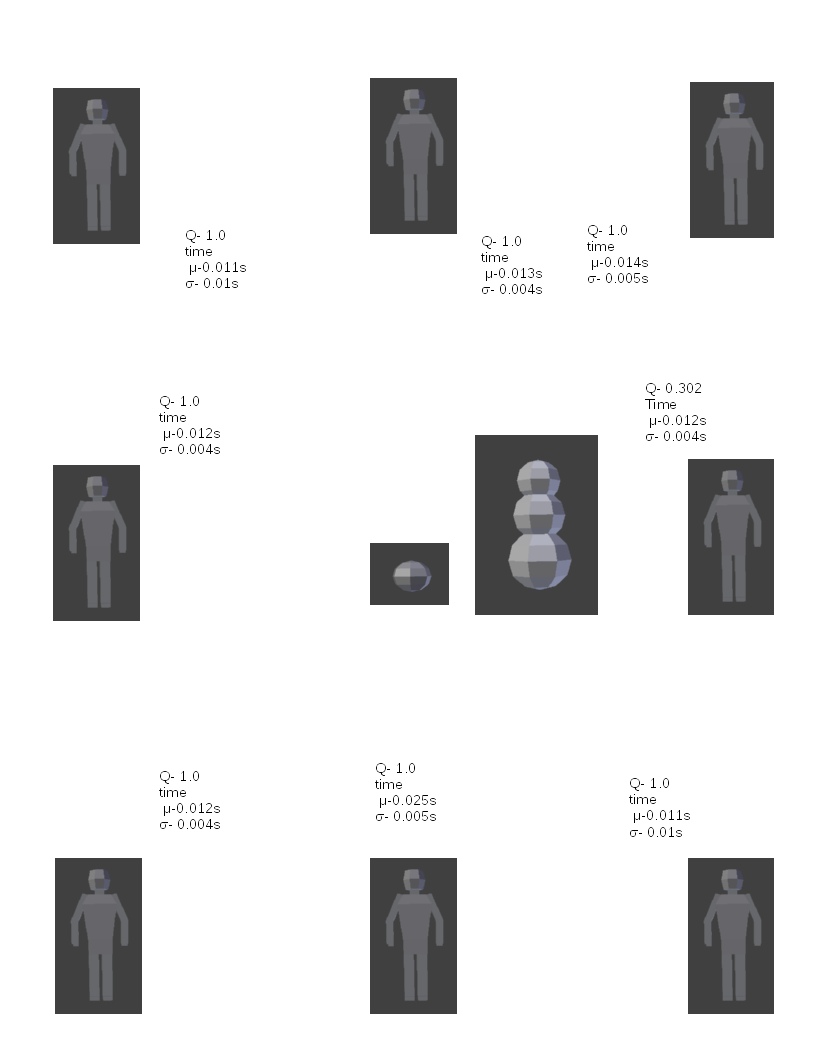
\includegraphics[width=0.75\textwidth]{figures/see_query.png}
	\end{center}
	\caption{In a variety of locations, \TDS is able to gauge visibility given the presence of obscuring objects. The relative locations of the snowman, ball, and person represent their location in the testing on the xy plane}
	\label{fig:see_query}
\end{figure}

As can be see in figure \ref{fig:see_query}, all spots have perfectly clear sight of the ball in the center, except for the one which is blocked by the snowman, which returns a reduced sight capacity. This demonstrates the vision capabilities of the system, and the degree to which the occlusion feature accurately simulates reality.

\section{Binary Placement Testing}

Placement testing began with the placement of objects in a scene with one predication. All of the predications were tested, and the person and ball objects were used, so that the predications all took the form:
\begin{center} \texttt{<predicate>(A,B)}\end{center}

Every predication was tested twenty times, ten times with each object as the focal object.

The placement function's rejection sampling was also tested for efficiency. Tests were done with no threshold (no rejection sampling), low threshold (placements had to return a non-zero query value), and high threshold (placements had to return a query satisfaction of at least $0.25$). It was noted that for threshold values greater than this, the program failed to terminate in reasonable time (less than 5 minutes). 

Figure \ref{fig:binary_place_ballAndPerson_noThresh} shows the results of the first round of tests, placement with no rejection sampling. 

\begin{figure}[h]
	\begin{center}
		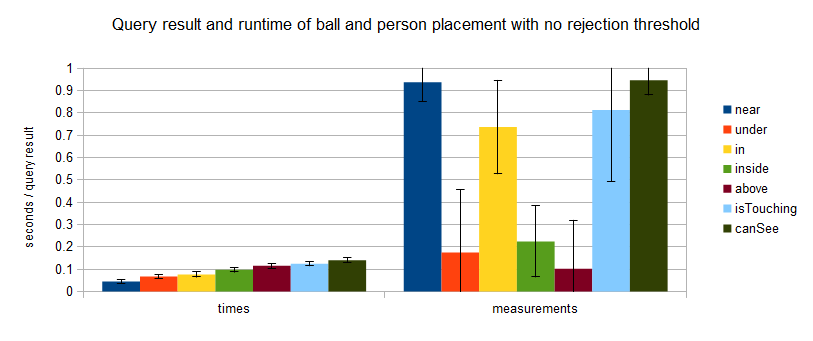
\includegraphics[width=0.8\textwidth]{figures/binary_place_ballAndPerson_noThresh.png}
	\end{center}
	\caption{Placement with no rejection sampling. \texttt{Near}, \texttt{isTouching}, \texttt{canSee}, and \texttt{in} all show accurate placement, while others do not. Considerable variation is present amongst all predicates.}
	\label{fig:binary_place_ballAndPerson_noThresh}
\end{figure}

The results give a good indication of the satisfiability of the placement areas returned by the placement functions. Because the areas where the \texttt{near}, \texttt{in}, \texttt{isTouching}, and \texttt{canSee} predications hold are represented accurately (in a scene with two objects) by the valid placement returned by the placement function. The remaining predicates, however, are not very well represented by these placement areas, and as such their average satisfaction is much lower.

The test for a low threshold are represented in figure \ref{fig:binary_place_ballAndPerson_lowThresh}. 

\begin{figure}[h]
	\begin{center}
		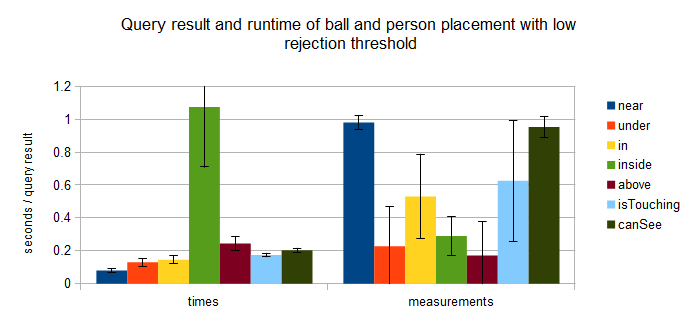
\includegraphics[width=0.8\textwidth]{figures/binary_place_ballAndPerson_lowThresh.png}
	\end{center}
	\caption{Placement with low rejection sampling. Slight but not significant improvements are shown across all predicates, as well as a dramatic increase in run-time for the \texttt{inside} predicate.}
	\label{fig:binary_place_ballAndPerson_lowThresh}
\end{figure}

As can be seen by these results, there is a small but noticeable trade-off for all predications. As before there is a high amount of variance for predications whose placement areas do not match their query-satisfaction areas closely. For most, the difference between the results of this and the previous experiment are not significant, with the variations within one standard deviation. 

The one exception with this is the time for the inside predicate. The average time for this predicate is significantly longer than the others, so much so that it alters the scale of the graph.This provides evidence that the querying function for this predication is notedly more inefficient than the others.

The final tests were done with a high threshold, these results are shown in figure \ref{fig:binary_place_ballAndPerson_highThresh}.
\begin{figure}[h]
	\begin{center}
		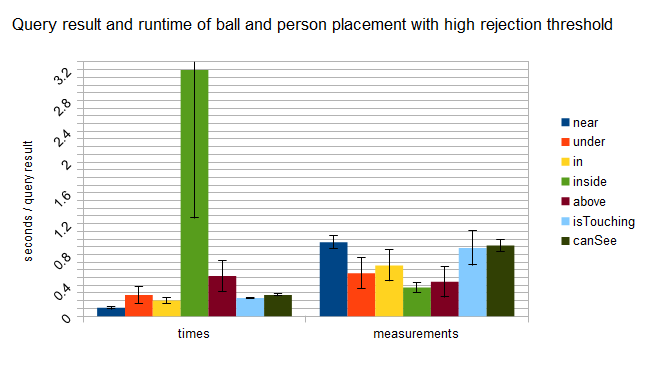
\includegraphics[width=0.8\textwidth]{figures/binary_place_ballAndPerson_highThresh.png}
	\end{center}
	\caption{Placement with high rejection sampling. Improvements are noticed in placement accuracy, though the run-time of the near predication increases even more dramatically then before.}
	\label{fig:binary_place_ballAndPerson_highThresh}
\end{figure}
In this graph we see more noted improvements within the code, particularly for the predications with higher variation in previous tests. The trade-off for most predicates was expected. However, as before, the inside predication's query time was increased considerably. It is reasonable to state that this predication has the longest run-time of any in the library, and that it is likely the limiting factor that prevents the system from terminating in reasonable time when a high rejection threshold is used.

\section{Full Scene Simulation}
Because the most important part of the project was to simulate the story scene featuring a boy and a girl seeing a bird's nest this, this scene became the staple for testing scenes with multiple objects and predications.
More specifically, this scene consisted of the following information:
\begin{itemize}
	\item Entities
	\begin{itemize}
		\item person ``A'' 
		\item tree ``B''
		\item nest ``C''
		\item egg ``D''
	\end{itemize}
	
	\item Predications 
	\begin{itemize}
		\item under(A,B)
		\item canSee(A,C)
		\item in(D,C)
		\item in(C,B)
	\end{itemize}
\end{itemize}

This corresponds to a simplified version of the story in the scene: one in which there is an egg in a nest (which is itself in a tree) and a child under the tree who can see the nest. 

Once the scene was constructed, the scene was queried to see if the person could both see the nest and the egg. Note that the person was placed in the scene \emph{without} the ``canSee(A,D)'' predication, and as such the scene was only configured such that the person could see the nest.
Because of this, and because the person was to be placed under the tree, it was highly unlikely that the person should be able to see the egg in the nest. Since the egg was completely on top of the nest, the person could only look up from below, and the nest is a completely opaque object (having occlusion of -1).

\begin{table}[h]
	\centering
	\begin{tabular}{|l c r|}
		\hline
		canSee egg&	canSee nest&	time\\\hline
		0&	0.6947030267&	137.34\\
		0&	0.998120801&	20.45\\
		0&	0.9678805377&	0.45\\
		0&	0.8965050001&	13.61\\
		0&	0.7376654109&	710.13\\
		0&	0.9193492216&	229.36\\
		0.0940467865&	0.8770202952&	2.84\\
		0&	0.5460023627&	11.99\\
		0&	0.9322889931&	36.05\\
		0&	0.9973411794&	23.23\\
		\hline\hline
		\multicolumn{3}{|l|}{averages}\\		
		0.0104496429&	0.874685978&	116.4566666667 \\\hline
		\multicolumn{3}{|l|}{standard deviation} \\
		0.0297402052&	0.1493400827&	220.5594981582
		\\\hline
	\end{tabular}
	\caption{The testing results for the story placement scene.}
	\label{table:story_placements}
\end{table}
The results of the test, including the placement and subsequent querying, are displayed in figure \ref{table:story_placements}. In all but one test, the system was able to correctly place the objects in the scene in such a way that the person was able to see the nest, but not the egg inside. This indicates a very high rate of success for the IMS's predication placement and querying setup. It should also be noted that variability in the visibility of the nest is a result of the nest being placed inside the tree canopy, which has an opacity of $0.5$.